\chapter{Choosing a Prediction Model}
\thispagestyle{nohead}
\label{Prediction}

This chapter will evaluate the effectiveness of a number of machine learning algorithms at predicting the most appropriate SMT solver to use on any (unseen) \why~PO.
Our goal in this thesis is to construct a ``meta-solver'' or \textit{portfolio} solver which chooses from a range of tools in order to prove more goals than a single solver is capable of.
We motivate the need for a portfolio solver with an analysis of our dataset 
in Sec. \ref{sec:portfolio-benefit}. 
More details about the type of prediction task chosen for the evaluation of ML algorithms is given in Sec. \ref{sec:reg-class}, with an introduction to a number of theoretical strategies chosen for comparison in Sec. \ref{sec:strategies}. A more detailed introduction to the six prediction models (introduced previously in Sec. \ref{sub:lrsvmmml} and Table \ref{table:algorithms}) is given in Sec. \ref{pred:choosing} before the results of their comparison is discussed. We end this chapter with a more detailed look at the model chosen for use in the actual implementation of \where~.

\section{The benefit of portfolio-solving in \why}
\label{sec:portfolio-benefit}

\newcolumntype{Z}{>{\raggedleft\arraybackslash}X} 
\begin{table}
	\caption[Results of running 8 solvers on the example \why~programs]{Results of running 8 solvers on the example \why~programs.  Also included is a theoretical solver  $ \mathcal{TS}$, which always returns the best answer in the fastest time.}
	\begin{tabularx}{1.1\textwidth}{@{}l|ZZZ|ZZZ|ZZZ@{}}
		\toprule
		{} & \multicolumn{3}{c|}{\textbf{File}} & \multicolumn{3}{c|}{\textbf{Theory}} & \multicolumn{3}{c}{\textbf{Goal}} \\
		{} & \# proved & \% proved & Avg time & \# proved & \% proved & Avg time & \# proved & \% proved & Avg time \\
		\midrule
		$ \mathcal{TS}$ & \textbf{48} & \textbf{37.5\%} & \textbf{1.90} & \textbf{190} & \textbf{63.8\%} & \textbf{1.03} & \textbf{837} & \textbf{79.9\%} & \textbf{0.42} \\
		\textbf{Alt-Ergo-0.95.2} & 25 & 19.5\% & 1.45 & 118 & 39.6\%& 0.77 & 568 & 54.2\% & 0.54 \\ 
		\textbf{Alt-Ergo-1.01} & 34 & 26.6\% & 1.70 & 142 & 47.7\% & 0.79 & 632 & 60.3\% & 0.48 \\ 
		\textbf{CVC3} & 19 & 14.8\% & 1.06 & 128 & 43.0\% & 0.65 & 597 & 57.0\% & 0.49 \\ 
		\textbf{CVC4} & 19  & 14.8\% & 1.09 & 117 & 39.3\% & 0.51 & 612 & 58.4\% & 0.37 \\ 
		\textbf{veriT} & 5 & 4.0\% & 0.12 & 79 & 26.5\% & 0.20 & 333 & 31.8\% & 0.26 \\ 
		\textbf{Yices} & 14 & 10.9\% & 0.53 & 102 & 34.2\% & 0.22 & 368 & 35.1\% & 0.22 \\ 
		\textbf{Z3-4.3.2} & 25 & 19.5\% & 0.56 & 128 & 43.0\% & 0.36 & 588 & 56.1\% & 0.38 \\ 
		\textbf{Z3-4.4.1} & 26 & 20.3\% & 0.58 & 130 & 43.6\% & 0.40 & 581 & 55.4\% & 0.35 \\ 
		\bottomrule
	\end{tabularx}
	\label{table:avgtimes}
\end{table} 


Now that the SMT solvers to be supported by \where~have been identified and an appropriate dataset for training and testing purposes has been chosen, we can make a preliminary and exploratory analysis of the behaviour of the SMT tools on the particular data. 
We aim to make a case for portfolio-solving as an effective method for discharging POs in the \why~system.

We refer the reader to Table \ref{table:avgtimes} which shows the results of running 8 solvers on the example \why~programs with a timeout value of 10 seconds. 
The entire dataset is used in this case. 
WhyML files are modularised as a number of \textit{theories}. The \why~IVL identifies the \textit{goals} which need to be proven in order for the theory (and in turn the entire file) to be verified as correct. 
Our dataset of 128 WhyML files consists of 289 theories, which in turn generate 1048 goals. 
Aside from the number of each modular construct proved by the solver (left sub-column), the percentage this number represents of the total is given (centre sub-column) and the average time taken to prove each construct (as measured using the process described in Sec. \ref{sub:confidence}) is given in the right sub-column. 

We show the results of proving a WhyML using its modular constructs as this method of verification is particularly useful when \why~is run in batch mode from the command line.
It is more natural to select separate solvers on a per-goal basis through the \why~IDE which breaks each WhyML program in to theories and goals automatically. 

Table \ref{table:avgtimes} also shows the results for a \underline{T}heoretical \underline{S}olver $ \mathcal{TS} $. 
$ \mathcal{TS} $ is the best solver, from the eight SMT solvers measured, chosen on a per-goal basis. 
For example, if a file contains one theory which consists of three goals, and the best-performing solver is CVC4 for the first goal, Yices for the second, and CVC3 for the third, the result for $\mathcal{TS}$ on that file is the sum of the results for CVC4 on the first goal, Yices on the second, etc.
We define what is means for a solver to be the \textit{best} in the next subsection.

It is important not to confuse $\mathcal{TS}$ with the theoretical \textsf{Best} ranking introduced in Sec. \ref{sub:best}. 
$\mathcal{TS}$ refers to a single solver (and hence is directly comparable to the other eight SMT solvers in Table \ref{table:avgtimes}), while \textsf{Best} refers to a \textit{ranking} which uses all eight solvers. $\mathcal{TS}$ is equivalent to using the top-ranking solver from \textsf{Best} and stopping.

The theoretical solver $\mathcal{TS}$ shows the benefit of being able to use the most appropriate solver for each PO: 205 more goals are provable -- an increase of 19.6\% -- over the best single solver (Alt-Ergo version 1.01) which can prove a total of 632. 
In total, 837 goals are provable by using a combination of the 8 solvers -- a figure that represents 79.9\% of the 1048 goals. 
$\mathcal{TS}$ proves goals in a shorter amount of time than either version of Alt-Ergo or CVC3, on average. 
The average time subcolumn provides an insight into how solvers which can prove relatively few goals, theories, or entire files -- such as veriT or Yices -- can be useful in a portfolio-solving context: such solvers often prove what they can in a very short amount of time (veriT take an average time of just 0.12 seconds, for example, to prove each of 5 entire files) and can be the best choice of solver for those files, theories and goals. 

\subsection{The relative utility of solver responses}
\label{sub:rel-util}

To make assertions about the relative performance of different solvers on the same goal, a definition of the relative \textit{utility} of solver responses is required.
Should a solver that returns an answer of \textit{Valid} in 5 seconds be seen as ``worse'' than one that returns \textit{Unknown} in 0.5 seconds? 
Likewise, should the solver returning \textit{Failure} after 1 second be penalised more severely than one returning \textit{Timeout} after the maximum time limit?

We define an ordering for response utility as 
\[
\lbrace Valid, Invalid\rbrace > Unknown > \lbrace Timeout, Failure\rbrace
\]  
the reasoning being that a \textit{Failure} response usually signals a fatal error in the logic encoding for that solver/goal pair, and the learning algorithm should be discouraged from choosing a failing solver for the particular goal characteristics in question. 
As discussed in Sec. \ref{sub:timeout-limit} of the previous chapter, \textit{Unknown} answers are returned quickly in general, and should not be penalised as much as \textit{Timeout} responses. 
Solvers which reach the timeout limit are unlikely to return a \textit{Valid} or \textit{Invalid} response give more time (illustrated clearly by Fig. \ref{fig:line_graph}).
Solvers returning the same answer are ranked according to runtime -- with faster solvers being preferred.

This method for defining relative performance has similarities to the scoring structure for ATPs competing in SV-COMP \cite{Beyer2016, SVCOMP}, with some important differences. 
Although the notion of ``false positive'' and ``false negative'' responses is not applicable in the SMT domain (where tools are assumed to be sound), a ``true positive'' (or \textit{Valid}) is scored marginally higher than a ``true negative'' (or \textit{Invalid}). 
In contrast, \textit{Unknown, Timeout} and \textit{Failure} responses are not treated separately by the SV-COMP model -- they all fall under the \textit{Unknown} response category and receive a score of zero.
%A further refinement to our scoring model was necessary in order for the prediction models to operate effectively. 
The definition of the \textit{cost} function we applied to solver results is given in Sec. \ref{sub:scoring} of this chapter. 

\section{Classification and regression}
\label{sec:reg-class}

Machine learning prediction tasks can be separated into two categories: those involving the \textit{classification} of a variable into discrete categories or classes, and those predicting a continuous-valued variable directly -- \textit{regression} tasks.
This section will discuss some of the options considered when designing \where's prediction task.

\subsection{Predicting the single best solver} This option involves a multi-class classification task: the classes involved are the eight SMT solvers.
Each PO is classified as belonging in one class. 
This direction was rejected as some benefits associated with portfolio-solving were lost: if the PO is misclassified, the performance of the portfolio solver suffers severely.
The single solver can return return an answer of \textit{Failure} and no other solver suggestion is made: this method was found to be only marginally better than choosing one of the eight solvers at random. 
\subsection{Predicting the best \textit{ranking} of solvers} Again, this option is a multi-class classification task. 
Instead of predicting a single solver, however, the task involves predicting the entire ranking of eight solvers. 
The benefit of obtaining a ranking is the flexibility it affords in calling SMT solvers sequentially or in parallel.
If the first solver fails or returns a answer other than \textit{Valid} or \textit{Invalid}, the next best predicted solver is called, and so on.
With 8 SMT solvers there are 8! (or 40,320) rankings -- far too many to be reasonable for a classification task -- leading to this approach being rejected.
Many of these rankings were observed very rarely or did not appear at all in the training data. 
Such an unbalanced dataset is not appropriate for accurate classification.
\subsection{Predicting solver runtime and response separately}
This approach involves two separate tasks, each predicting a characteristic of the solver's performance. 
One algorithm would attempt to predict the response class (i.e. \textit{Valid, Invalid}, etc.) while another would attempt to predict the solver runtime.
The former task is a multi-class classification task with five classes, while the latter is a multi-output regression task.
This method has the advantage of affording the user flexibility in how to choose the ultimate ranking: if fast responses are preferred over \textit{Valid} answers.
This flexibility comes at the price of complexity, however: two accurate predictors, a classifier and regressor, are required instead of one.
\subsection{Combining the prediction of solver response and runtime}
This option uses a cost function to combine the two solver response variables as a single real-valued number which is used for ranking the solvers.
This is a multi-output regression task: a cost prediction is made for each solver individually.
The individual predicted values are sorted in increasing order to produce a ranking of decreasing ``solver utility''.
This approach shares most of the advantages of predicting solver response and runtime separately: each solver's actual behaviour is predicted directly rather than the relative behaviour of all eight \textit{together} constituting a single class. 
It is relatively simple to change the cost function, although it can not be done ``on-the-fly'' in the same manner as the previous approach.
A change to the cost function requires re-training the model.
The major benefit is having one single model to predict both the solver response and the runtime. 
This is the prediction approach chosen for \where~in this thesis.  

\subsection{The Cost Function}
\label{sub:scoring}

The cost function should reflect the ordering of solver utility defined in Sec. \ref{sub:rel-util}: penalising poorly-performing solvers while ensuring \textit{Valid} and \textit{Invalid} response incur the lowest cost.
The following simple function allocates a cost to each solver $S$'s response $\langle answer, time\rangle$ to each goal $G$:
\[\small
cost(S,G) = 
\begin{cases}
time_{S,G}, \text{ if answer}_{S,G} \in \lbrace Valid, Invalid \rbrace \\
time_{S,G} + \text{timeout}, \text{ if answer}_{S,G} = Unknown \\
time_{S,G} + (\text{timeout} \times 2), \text{ if answer}_{S,G} \in \lbrace Timeout, Failure \rbrace
%dist((time_{S,G},\text{timeout}), (0,0)), \text{if answer}_{S,G} \in \lbrace Timeout, Failure \rbrace
\end{cases}
\]
Thus, to penalise the solvers that return an \textit{Unknown} result, the timeout limit is added to the time taken, while solvers returning \textit{Timeout} or \textit{Failure} are further penalised by 
adding double the timeout limit to the time taken.
A response of \textit{Failure} refers to an error with the back-end solver and usually means a required logical theory is not supported. 
This function ensures the best-performing solvers always have the lowest costs. A ranking of solvers for each goal in order of decreasing relevance is obtained by sorting the solvers by ascending cost.\\ 
\\


\begin{table}
	\caption[Result of 8 solver executions on \textit{first\_last} ]{Result of 8 solver executions on \textit{first\_last}}
	\begin{tabularx}{\textwidth}{@{}YYYYYY@{}}
		\toprule
		\textsc{Solver} & \textsc{Version} &  \textsc{Runtime (Secs)} & \textsc{Response} & \textsc{Cost} & \textsc{Rank Position} \\
		\midrule
		Alt-Ergo & 	0.95.1 & 	0.134 & 	Unknown & 	10.134 & 2\\
		Alt-Ergo & 	1.10 & 		0.170 & 	Unknown & 	10.171 & 3\\
		CVC3 & 		2.4.1 & 	0.356 & 	Valid & 	0.356 & 1\\
		CVC4 & 		1.4 &		0.173 & 	Unknown  & 	10.173 & 4\\
		veriT & 	201506 & 	10.109 & 	Timeout & 	30.109 & 5\\
		Yices & 	1.0.38 & 	10.161 & 	Timeout & 	30.161 & 8\\
		Z3 & 		4.3.2 & 	10.115 & 	Timeout & 	30.115 & 6\\
		Z3 & 		4.4.1 & 	10.131 & 	Timeout & 	30.131 & 7\\
		%	\midrule
		%	\multicolumn{3}{l}{\textsc{Derived Ranking}:} & & & \\
		%	\multicolumn{4}{l}{CVC3 > Alt-Ergo-0.95.1 > Alt-Ergo-1.01 >} & & \\
		%	& & \multicolumn{4}{r}{CVC4 > veriT > Z3-4.3.2 > Z3-4.4.1 > Yices}  \\
		\bottomrule
		
	\end{tabularx}
	\label{table:cost}
\end{table}
\textbf{Example: using the cost function to obtain a ranking for \textit{first\_last}}: \\
To illustrate the effect of applying our cost function, we return to the \textit{first\_last} goal introduced in the previous chapter.
Table \ref{table:cost} lists the results of executing the 8 solvers on the goal, as measured using the method described in Sec. \ref{sec:dependant}. 
The derived cost value for each solver is used as its dependent variable in the prediction models compared in Sec. \ref{pred:choosing} and \where~'s actual implementation  



\section{Ranking strategies}
\label{sec:strategies}

As discussed in relation to $\mathcal{TS}$, rankings are not directly comparable to single solvers. 
The following theoretical ranking strategies provide a basis by which we can compare and evaluate the solver rankings predicted by the ML models.
The \textsf{Best} and \textsf{Worst} strategies use the empirical measurements to construct rankings on a per-goal basis, while the \textsf{Random} strategy uses the same set of rankings for each goal.
We refer to the following strategies as \textit{theoretical} as they assume knowledge of the actual behaviour of the solvers for the goal in question -- knowledge which is impossible to have prior to execution in a real-world verification scenario.     

Algorithm \ref{algo:rank} describes the process used by solver rankings to return answers and runtimes. This process is used in our algorithm comparison and \where~'s evaluation.
Essentially, the runtime of next best solver (according to a given ranking) is added to the cumulative total until an answer of \textit{Valid} or \textit{Invalid} is returned or the array of solvers has been exhausted. 
When solver answers are compared in the \texttt{if} statement, the following relative value of answers is used: $Valid > Invalid > Unknown > Timeout > Failure$.

\begin{algorithm}
	\caption{Returning answers and runtimes from solver rankings}
	\KwIn{Solvers $\lbrace S_1,...,S_n\rbrace$ sorted by cost (predicted, actual, or random)}
	\KwOut{$\langle A,T\rangle$ where $A$ = the best answer from the solvers; $T$ = the cumulative time taken to return $A$}
	\Begin{
		\tcp{initialisation}
		$A \leftarrow Failure$ \\
		$T \leftarrow 0$ \\
		$i \leftarrow 1$ \\
		\While{$A \notin \lbrace Valid, Invalid \rbrace \wedge i \leq n$}
		{$A_S \leftarrow Answer(S_i)$ \tcp{the answer returned by solver $S_i$
			}
			$T \leftarrow T + Time(S_i)$ \tcp{add solver $S_i$'s time to the cumulative runtime}
			\If{$A_S > A$}{$A \leftarrow A_S$ \tcp{$S_i$'s answer is better than the current best answer}}
			$i \leftarrow i + 1$}
		\Return{$\langle A,T\rangle$}} 
	\label{algo:rank}
	
\end{algorithm}

\subsection{\textsf{Best}}
\label{sub:best}

The \textsf{Best} ranking is the one derived from sorting the solvers in terms of increasing cost. 
Referring to the solver costs listed in Table \ref{table:cost}, the \textsf{Best} ranking for this goal is
CVC3 > Alt-Ergo-0.95.1 > Alt-Ergo-1.01 > CVC4 > veriT > Z3-4.3.2 > Z3-4.4.1 > Yices. 
As the first-choice solver according to this ranking -- CVC3 -- returns an answer of \textit{Valid}, no other solver will be called after the first returns its answer. 
Thus for the \textit{first\_last} goal, the \textsf{Best} ranking strategy returns an answer of \textsf{Valid} in 0.356 seconds.   

\subsection{\textsf{Worst}}

The \textsf{Worst} ranking is the inverse to the \textsf{Best}. 
For the \textit{first\_last} goal, Yices will be the first solver called by this strategy.
As Yices returns an answer other than \textit{Valid} or \textit{Invalid}, the next solver in the ranking (Z3 version 4.4.1) will called, and so on.
The user of this strategy would have to wait until the eighth solver, but a \textit{Valid} answer would eventually be returned.
For the example goal, the \textsf{Worst} strategy returns an answer of \textit{Valid} in 41.349 seconds.

Both the \textsf{Best} and \textsf{Worst} strategies provide important upper and lower bounds for a strategy's runtime.
If a goal is provable by any of the eight solvers, any of our theoretical strategies will be able to prove it.
The difference between these strategies is how long the goal takes to be proven.  

\subsection{\textsf{Random}}

The \textsf{Random} strategy differs from the previous two because it does not refer to \textit{one} ranking but to \textit{all possible} rankings.
The set of all possible rankings is the same for all goals, but the the runtime and result obviously vary. 
The runtime associated with the \textsf{Random} strategy is the average runtime for the 8! or 40,320 possible solver rankings.
For the \textit{first\_last} goal, the \textsf{Random} strategy returns an answer of \textit{Valid} in 20.853 seconds.

\section{Choosing the most effective prediction algorithm}
\label{pred:choosing}
\begin{figure}
	\centering
	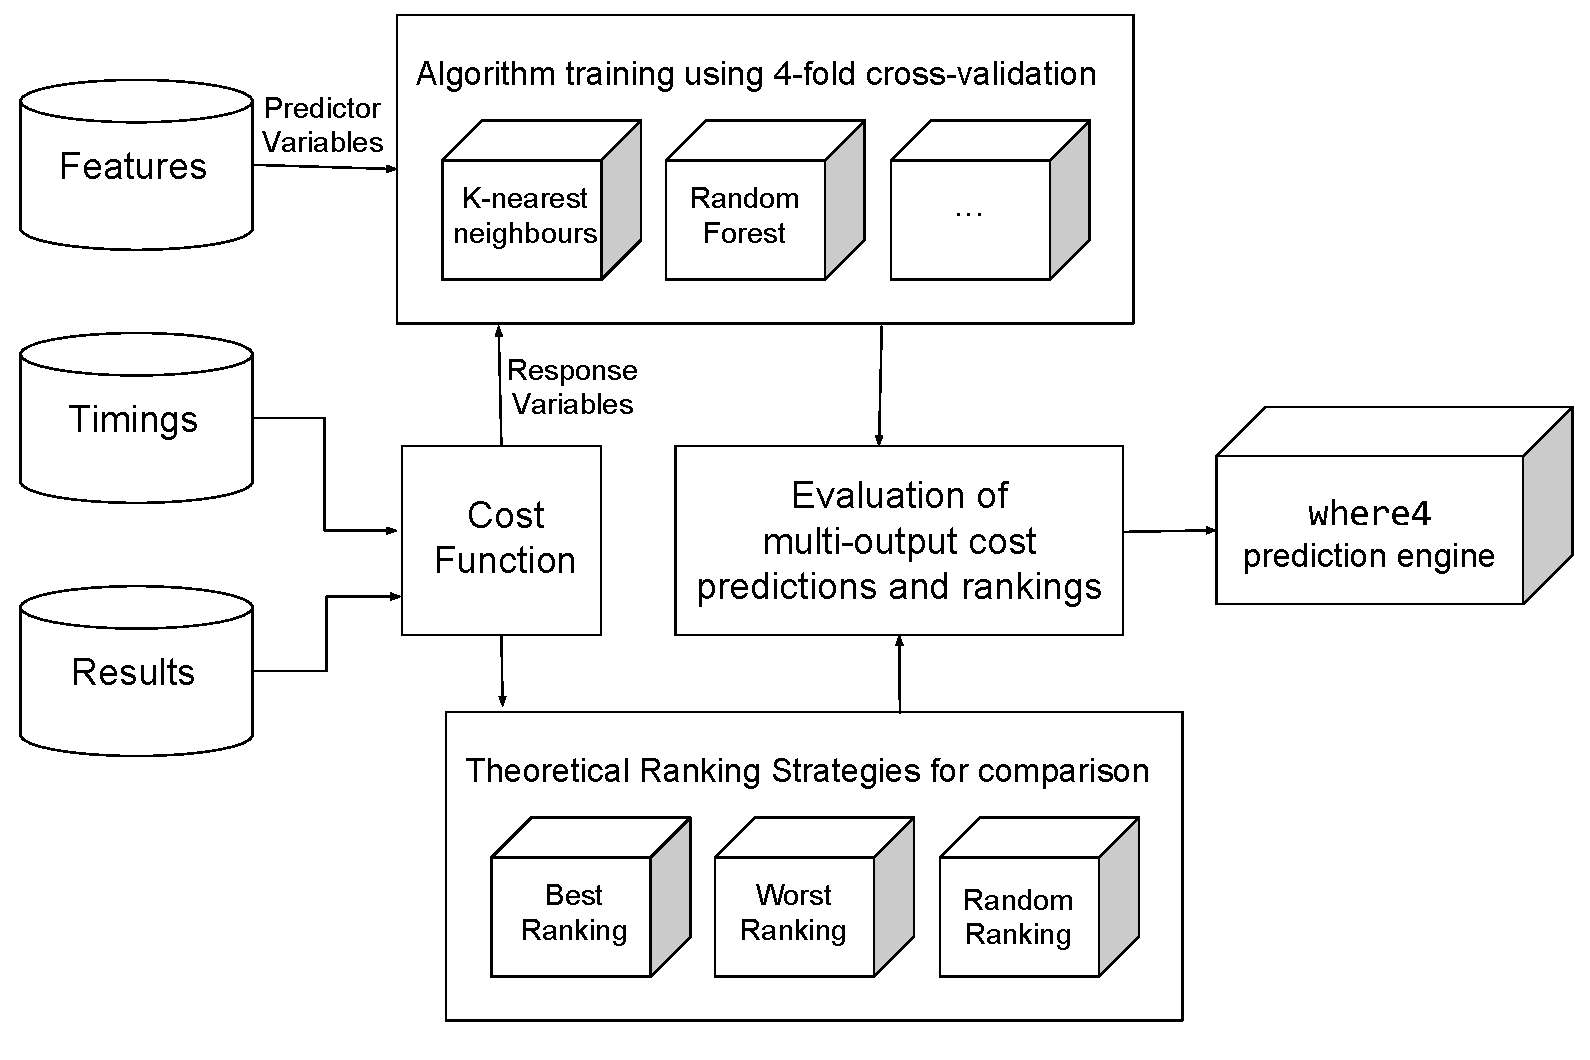
\includegraphics[width=0.9\linewidth]{Figures/Chapter4}
	\caption{Overview of the process used to derive the \where~prediction model}
	\label{fig:Chapter4}
\end{figure}

Fig. \ref{fig:Chapter4} illustrates a high-level view of the process used to compare and evaluate the various ranking strategies in this section. 
The solver timings and results are combined as a single variable using the cost function defined in Sec. \ref{sub:scoring}.
The value returned by this function is the response variable for a number of ML algorithms; with the statically-extracted features acting as the predictor variables.

A four-fold cross validation of this data is used to evaluate the models. 
In this method, the data is split into quarters.
Four models are trained on different dataset by holding a different quarter back for model evaluation each time.
The final evaluation is based on the model's average performance over the four instances.
\textit{K-fold} cross validation allows the use of the entire dataset for model evaluation and training (rather than holding a portion of the data back solely for model evaluation use -- a technique known as ``hold-out'' validation).   

\subsection{Evaluated models}

The ML algorithms compared in this section have briefly introduced in Sec. \ref{sub:lrsvmmml}. 
In this section, we go into more detail about how the algorithms operate and the specific variants and parameters chosen for use during this model comparison.
We used the Sci-Kit Learn \cite{sklearn} Python implementation for all algorithms.
The library is well documented and the consistent API is well-designed. 



\subsubsection{Support Vector Machines}

As a member of the \textit{analogical} family of learning algorithms, Support Vector Machines (SVMs) \cite{svm} are based on a concept of similarity between training instances. 
During training, a number of separating hyperplanes are determined.
The idea behind SVMs is to ensure the distance from this hyperplane to any training instances closest to it is maximal.
This process is known as ``maximising the margin'' and is designed give the model the best chance at classifying unseen instances correctly. 
The set of training instances closest to the margin is called the \textit{support vector} as they can be thought of as ``holding up'' the hyperplane.

A number of kernel functions can be used as a similarity measure during training.
We chose to use the \textit{Radial Bias Function} (RBF) kernel as we can not assume a linear relationship between our features and cost value. 
The RBF kernel requires the use of two hyperparameters to control how flexible the model is (i.e. how closely is fits the training data). 
We used a grid search technique \cite{hsu2003practical} to identify the $C$ (hyperplace smoothness) and $gamma$ (the radius of influence for each individual training instance) parameters.

In the multi-output case, each cost value has to be predicted individually for each solver -- requiring the use of 8 SVMs each tuned to different parameters on a per-solver basis.
The benefit of using SVMs is their ability to give good results in large-dimensional spaces; even with large datasets. 

\subsubsection{Decision Trees}

Decision trees \cite{DecisionTrees} work by constructing a binary tree; recursively splitting the data by the feature and threshold which create the most distinct partitions.
Features of new instances are queried according to the thresholds specified by the non-leaf nodes, with leaves consisting of (one or many) predictions. 
The original implementation required that features be categorical (Quinlan's ID3 algorithm). 
Sci-kit Learn uses the CART \cite{cart} algorithm which supports numerical features and outputs for regression tasks.  

Decision trees are a transparent and powerful method for classification and regression.
Since the 1960s, decision trees have been successfully deployed in many domains. 
In the intervening years, techniques have been developed to improve the accuracy and generalisability of decision trees: such techniques include pruning of \textit{if-then} branches created by sequences of splitting nodes, and termination conditions such as limiting the depth of the tree and making each leaf node account for a minimum number of examples in the training data.
We chose this last technique as a method to prevent our decision tree from overfitting training data: a minimum of five training instances had to be described by the \textit{if-then} rule associated with the leaf.
This constraint has the effect of combining nodes which use splitting rules to produce leaves smaller than size five; using them as leaves instead. 

\subsubsection{Random Forests}

Random forests \cite{RandomForests} were created as a response to decision tree's tendency to overfit training data -- leading to poor generalisation results.
As the name suggests, this technique involves creating many decision trees, with each tree trained on a random subset of the training data and/or restricted to using a subset of the features for use in splitting nodes.
Random forests are an example of an \textit{ensemble} method which uses multiple weak predictors to strengthen the overall prediction.

For classification problems, each tree ``votes'' on an instance's class.
In the regression case, all trees' predictions are averaged to determine the forest's ultimate prediction.   

Similar to our use of decision trees, we limited the depth of each tree by specifying a minimum size of five for each leaf node. 
We used 100 trees in the random forest.

\subsubsection{Linear and Ridge Regression} 

Linear regression attempts to predict the parameters of a function which fits the input features to the output variable. 
It expects that the output variable be a linear combination of the input variables.
We used the Ordinary Least Squares formulation which attempts to minimise the sum of squared error for the set of training instances to the output variable.    

Ridge regression \cite{ridge} is a generalised linear model which attempts to be more robust to violations in the input variables' independence. 

\subsubsection{K-Nearest Neighbours Clustering}

K-Nearest Neighbours clustering, like SVMs, belong to the analogical family of predictors which rely on a similarity measure to group training instances (we used the standard Euclidean distance).
The idea is to create $K$ clusters of training instances which are ``most similar'' to each other in terms of features -- with each feature acting as a dimension.   
In contrast to SVMs however, most clustering algorithms (K-nn included) do not scale well in high-dimensional spaces.

Typically used for classification tasks, the K-nn algorithm can be adapted for regression by calculating the target/response variable as the average of all instances in its cluster.
We used a modification: training instances ``closer'' to the unseen instances are weighted more than those further away in the cluster when computing the target variable.
This variation makes the algorithm more robust to noisy training data. 


\subsection{Train / Test Split}

In the previous chapter, we described our dataset as consisting of 1048 \why~POs.
We now split this dataset into two disjoint subsets: the \textit{training} and \textit{testing} sets. 
The rest of this chapter uses only the \textit{training} set while the \textit{testing} set is used in our final evaluation of \where~in Chapter \ref{Evaluation}.

The training set represents 75\% of the entire dataset: 96 files,   212 theories and 785 goals. 
The data was split on a per-file basis to ensure that the no PO in the training set belonged to the same theory or file as a PO in the test set. 


\subsection{Cost discretisation}

Beside the standard implementation of the prediction algorithm, two variations were evaluated: cost discretisation and instance weighting (Sec. \ref{sub:weighting}).
By discretisation we describe the process to transform a continuous-valued variable into one of a finite number of values. 
It usually involves dividing variable by some small empirically-tested number. 

Discretisation allows algorithms which perform better when given a smaller number of discrete options for prediction to be identified. 
We chose 2.5 to be a discretisation divisor for the response variable (i.e. each solver's cost).
In choosing this value, it was important to minimise the discretisation error inherent in the process with a relatively small number of possibilities for prediction.

\subsection{Instance Weighting}

\label{sub:weighting}

The other technique we applied during predictor evaluation was the weighting of training instances.
Weighting is standard practice in supervised machine learning: each instances's weight was defined as the standard deviation of solver costs. 
This function was designed to give more importance to instances where there was a large difference in performance among the solvers; thereby de-emphasising trivial POs provable by most or all solvers, and empirically hard instances for which all solvers fail or time out.  

Note that the Sci-kit Learn implementation of K-Nearest Neighbours does not support instance weighting.

\subsection{Evaluation metrics}


\begin{table}
	\caption[Predictor Selection Results]{ Predictor Selection Results. * indicates the best result among the prediction models }
	
	\begin{adjustbox}{angle=90} 
		\begin{tabularx}{0.9\textheight}{@{}lrrZZZZZ@{}}
			{} & \textbf{Discretised} & \textbf{Weighted} & \textbf{Time (secs)} &  \textbf{nDCG} &  $R^2$ &  \textbf{MAE} &  \textbf{Reg-error} \\
			\midrule
			\textsf{Best}  &  &                             &     12.63 &   1.00 &   - & 0.00 &        0.00 \\
			\textsf{Random} & &                           &     19.06 &  0.36 &   - & 2.62 &       50.77 \\
			\textsf{Worst}  & &                           &     30.26 &  0.00 &   - & 4.00 &       94.65 \\
			\midrule
			\multirow{4}{*}{Decision Tree}  & \xmark & \xmark     &     15.80 &  0.50 &   0.11 & 2.06 &       43.12 \\
			  & \cmark & \xmark     &     15.84 &  0.43 &  -0.17 & 2.31 &       43.67 \\
			 & \xmark & \cmark     &     16.29 &  0.48 &  -0.12 & 2.10 &       45.09 \\
			 & \cmark & \cmark &     16.35 &  0.42 &  -0.18 & 2.28 &       45.03 \\
			\midrule
			\multirow{2}{*}{K-Nearest Neighbours} & \xmark & \xmark          &     15.93 &  \textbf{*0.53} &   0.16 & \textbf{*2.00} &       43.41 \\
			 & \cmark & \xmark          &     15.87 &  0.42 &  -0.18 & 2.32 &       43.24 \\
			\midrule
			\multirow{4}{*}{Linear Regression}  & \xmark & \xmark                        &     15.17 &  0.42 &  -0.16 & 2.45 &       49.25 \\
			 & \cmark & \xmark                     &     15.17 &  0.42 &  -0.29 & 2.46 &       49.28 \\
			 & \xmark & \cmark                 &     15.32 &  0.42 &  -0.41 & 2.44 &       48.71 \\
			 & \cmark & \cmark             &     15.35 &  0.41 &  -0.27 & 2.45 &       48.99 \\
			\midrule
			\multirow{4}{*}{Support Vector Regressor}  & \xmark & \xmark                           &     15.57 &  0.47 &   0.14 & 2.26 &       47.45 \\
			  & \cmark & \xmark                        &     15.43 &  0.43 &  -0.24 & 2.31 &       44.17 \\
			  & \xmark & \cmark                    &     15.61 &  0.47 &  -0.06 & 2.19 &       42.86 \\
			 & \cmark & \cmark                &     15.70 &  0.45 &  -0.20 & 2.23 &       43.34 \\
			\midrule
			\multirow{4}{*}{Random Forest}   & \xmark & \xmark         &     15.02 &  0.48 &   \textbf{*0.28} & 2.08 &       \textbf{*38.91} \\
			 & \cmark & \xmark         &     \textbf{*14.92} &  0.48 &  -0.18 & 2.13 &       39.19 \\
			 & \xmark & \cmark     &     15.06 &  0.48 &   0.18 & 2.12 &       39.46 \\
			 & \cmark & \cmark &     15.09 &  0.48 &  -0.16 & 2.15 &       39.18 \\
			\midrule
			\multirow{4}{*}{Ridge Regression}  & \xmark & \xmark                          &     15.11 &  0.42 &  -0.15 & 2.45 &       49.09 \\
			 & \cmark & \xmark                         &     15.14 &  0.41 &  -0.29 & 2.46 &       49.29 \\
			 & \xmark & \cmark                     &     15.02 &  0.41 &  -0.21 & 2.48 &       50.15 \\
			 & \cmark & \cmark                 &     15.03 &  0.41 &  -0.23 & 2.49 &       50.09 \\
			
		\end{tabularx}
	\end{adjustbox}
	\label{table:predselection}
\end{table}

We refer the reader to Table \ref{table:predselection}. 
Results for all prediction algorithms are listed (with discretised and/or weighted variants where applicable) and compared with the three theoretical ranking strategies introduced in Sec. \ref{sec:strategies}.
For each of the five evaluation metrics, the best-performing algorithm is marked in bold with an asterisk. 

The first result column, labelled \textbf{Time (secs)}, shows the average time taken for the algorithm/strategy to return a \textit{Valid} / \textit{Invalid} response (if such a response was in the set of solver answers -- see Algorithm \ref{algo:rank}).

The next three columns' metrics are introduced in the three subsections to follow.

The rightmost column lists the average regression error per instance. 
We illustrate this metric with a small example. For two testing instances, the predicted and actual costs for three solvers are: 
\[ \left( \begin{array}{ccc}
0.5 & 10.0 & 5.0 \\
0.4 & 5.5 & 10.0  \end{array} \right) = \text{predicted};
\left( \begin{array}{ccc}
0.6 & 9.0 & 8.0 \\
0.7 & 9.5 & 7.0 \end{array} \right) = \text{actual}\]
which gives a per-instance regression error of
\[ \left( \begin{array}{c}
0.1 + 1.0 + 3.0 \\
0.3 + 4.0 + 3.0
\end{array}  \right) = 
\left( \begin{array}{c}
4.1 \\
7.3
\end{array}  \right) \] 
taking the average of the two instances' regression error, 4.1 and 7.3, gives 5.7.
It is this average error between predicted cost and actual cost for eight solvers which is listed in the rightmost column.

This particular metric may be treated with a note of caution, however, as the relative ranking of solvers -- which we argue is the most important prediction -- is not explicitly taken into account.
Note that when the predictions and actual costs are sorted in increasing order the best-performing solver is predicted correctly for both instances in the previous example.
The entire ranking of solvers is predicted correctly in the first instance.

The next subsection will describe a metric specifically designed to measure the accuracy of predicted rankings.  
 
\subsubsection{Normalised Distributed Cumulative Gain}

\label{sub:ndcg}

The second numeric column of Table \ref{table:predselection} shows the 
Normalised Discounted Cumulative Gain (\textbf{nDCG}), which is commonly used to evaluate the accuracy of rankings in the search engine and e-commerce recommender system domains \cite{NDCG}. 
Here, emphasis is placed on correctly predicting items higher in the ranking. For a general ranking of length $p$, it is formulated as:
\begin{equation}
\small
nDCG_p = \frac{DCG_p}{IDCG_p}
\quad\text{ where }\quad
DCG_p = \sum_{i=1}^{p} \frac{2^{rel_i} - 1}{log_2(i+1)}
\label{eq:ndcg}
\end{equation}

where $rel_i$ refers to the relevance of element $i$ with regard to a ground truth ranking, and we take each solver's relevance to be inversely proportional to its rank index.  
In our case, $p = 8$ (the number of SMT solvers).  
The $DCG_p$ is normalised by dividing it by the maximum (or \textit{idealised}) value for ranks of length $p$, denoted $IDCG_p$. 
As our solver rankings are permutations of the ground truth (making $nDCG$ values of 0 impossible), the values in Table \ref{table:predselection} are further normalised to the range [0..1] using the lower $nDCG$ bound for ranks of length 8 -- found empirically to be 0.4394.

Again, we illustrate our use of this metric with a small example. 
Take a ground truth ranking or eight items sorted in decreasing relevance as
\[ A > B > C > D > E > F > G > H. \]
We take each item's \textit{relevance} to be inversely-proportional to its rank position:
\[rel_A=8, rel_B=7, rel_C=6, rel_D=5, rel_E=4, rel_F=3, rel_G=2, rel_H=1.\]
The predicted ranking of these items is
\[ B > A > C > F > D > E > G > H .\]
Applying Equation \ref{eq:ndcg} to these values gives us an $nDCG$ value of
\[
\frac{127}{1.0} + \frac{255}{1.58} + \frac{63}{2.0} + \frac{7}{2.32} + \frac{31}{2.58} + \frac{15}{2.81} + \frac{3}{3.0} + \frac{1}{3.17} = 341.053. 
\]
It can be shown that $IDCG_8 = 389.591$ which makes the un-normalised $nDCG$ value for the predicted ranking 0.875. Using the lower bound of 0.4394 to normalise this value to the range $\left[0, 1 \right]$ (accounting for permutations of length 8) gives us a final $nDCG$ score of 0.778. 

\subsubsection{$R^2$ Score}

The third numeric column of Table \ref{table:predselection} shows
the $R^2$ score (or coefficient of determination), which is an established metric for evaluating how well regression models can predict the variance of dependent/response variables. 
The maximum $R^2$ score is 1 but the minimum can be negative. Note that the theoretical strategies return rankings rather than individual solver costs. 
For this reason, $R^2$ scores are not applicable.

\subsubsection{Mean Average Error}

Table \ref{table:predselection}'s fourth numeric column shows the 
$MAE$ (Mean Average Error) -- a ranking metric which can also be used to measure string similarity. It measures the average distance from each predicted rank position to the solver's index in the ground truth.

Using the same predicted and actual rankings as Sec. \ref{sub:ndcg}, we calculate the $MAE$ to be:
\[
	MAE = \frac{1 + 1 + 0 + 2 + 1 + 1 + 0 + 0}{8} = 0.75
\]

\subsection{Properties of multi-output problems}
\label{sub:multi}

An interesting feature of all the best-performing models -- Random Forests, K-Nearest Neighbours, Decision Trees -- in Table \ref{table:predselection} is their ability to predict \textit{multi-output} variables \cite{multisurvey}. 
In contrast to the Support Vector model, for example, which must predict the cost for each solver individually, a multi-output model predicts each solver's cost simultaneously. 
Not only is this method more efficient (by reducing the number of estimators required), but it has the ability to account for the correlation of the response variables. 
This is a useful property in the software verification domain where certain goals are not provable and others are trivial for SMT solvers. 
Multiple versions of the same solver can also be expected to have highly correlated scores.

After inspecting the results for all learning algorithms (summarised in Table \ref{table:predselection}), we can see that Random Forests \cite{RandomForests} perform well, relative to other methods. 
They score highest for three out of 5 metrics (shown in bold) and have generally good scores in the others.

\section{The chosen model}
\label{sec:chosen}

